\documentclass[10 pt,usenames,dvipsnames, oneside]{article}
\usepackage{../../../modelo-ensino-medio}



\begin{document}

\begin{center}
  \begin{minipage}[l]{3cm}

\includegraphics[width=2cm]{logo}    
\end{minipage}\hfill
\begin{minipage}[r]{.8\textwidth}
 {\Large \scshape Atividade: Qual é a expressão?}  
\end{minipage}
\end{center}
\vspace{.2cm}

\ifdefined\prof
%Habilidades da BNCC
\begin{objetivos}
\item \textbf{EM13MAT304} Resolver e elaborar problemas com funções exponenciais nos quais é necessário compreender e interpretar a variação das grandezas envolvidas, em contextos como o da Matemática Financeira e o do crescimento de seres vivos microscópicos, entre outros. 
\end{objetivos}

%Caixa do Para o Professor
\begin{goals}
%Objetivos específicos
\begin{enumerate}
\item Deduzir expressões de funções exponenciais envolvendo expoentes racionais, a partir de situações problema.
\end{enumerate}

\tcblower

%Orientações e sugestões
\begin{itemize}
\item A ideia central é que se a cada $4$ dias o número de infectados triplica, a cada dois dias ficará multiplicado por $\sqrt{3}$, e cada $1$ dia ficará multiplicado por $\sqrt[4]{3}=\sqrt{\sqrt{3}}$. E isso levará à expressão $3^{\frac 14}$.

\item Como estamos propondo uma simulação de dados reais, é possível trabalhar com uma margem de aproximações para os valores colocados.

\item Ao término da atividade, durante as discussões, proponha algumas generalizações como: qual seria a fórmula se houvesse $200$ infectados no início? Se quintuplicasse a cada $4$ dias? Se quadruplicasse a cada $5$ dias? etc.
\end{itemize}
\end{goals}

\bigskip
\begin{center}
{\large \scshape Atividade}
\end{center}
\fi

Uma epidemia causada por um vírus está se espalhando na cidade. Os cientistas, após analisarem os primeiros dados concluem que a doença está se espalhando rapidamente porque o número de infectados está triplicando a cada $4$ dias. O número inicial de infectados que compuseram a análise foi de $100$ pessoas. Responda as perguntas.

\begin{enumerate}

\item{} Complete a tabela com os possíveis números de infectados observados pelos cientistas.

%\begin{figure}[H]
%\centering
%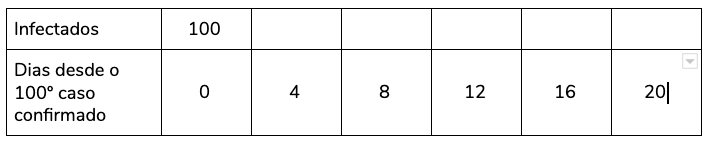
\includegraphics[width=300bp]{infectados.png}
%\end{figure}
\begin{center}
	\begin{tabular}{|c|c|c|c|c|c|c|}
		\hline
		\tcolor{Infectados}                                                                             & \tcolor{100} & \tcolor{}  & \tcolor{}  &  \tcolor{}  &  \tcolor{}  &  \tcolor{}  \\ \hline
		\begin{tabular}[c]{@{}c@{}}Dias desde o \\ $100^\circ$ caso \\ confirmado\end{tabular} & 0   & 4 & 8 & 12 & 16 & 20 \\ \hline
	\end{tabular}
\end{center}

\item{} Considerando que esse modelo retrata bem a realidade, ou seja, que a evolução do número de casos obedece a um padrão de crescimento exponencial, qual deve ser o número aproximado de infectados no segundo e no sexto dias desde o $100^\circ$ confirmado?

\begin{center}
	\begin{tabular}{|c|c|c|c|c|c|}
\hline
\tcolor{Infectados}                                                                    & \tcolor{100} & \tcolor{}  & \tcolor{}  & \tcolor{} \tcolor{} &  \tcolor{} \\ \hline
\begin{tabular}[c]{@{}c@{}}Dias desde o\\ $100^{\circ}$ caso\\ confirmado\end{tabular} & 0   & 2 & 4 & 6 & 8 \\ \hline
\end{tabular}
\end{center}

\item{} Complete a tabela abaixo,  com a possível evolução diária dos casos. Explique seu raciocínio.

\begin{center}
	\begin{tabular}{|c|c|c|c|c|c|l|l|l|l|}
\hline
\tcolor{Infectados}                                                                    & \tcolor{100} &  \tcolor{} & \tcolor{}  &  \tcolor{} & \tcolor{}  &  \tcolor{} & \tcolor{}  & \tcolor{}  &  \tcolor{} \\ \hline
\begin{tabular}[c]{@{}c@{}}Dias desde o\\ $100^{\circ}$ caso\\ confirmado\end{tabular} & 0   & 1 & 2 & 3 & 4 & 5 & 6 & 7 & 8 \\ \hline
\end{tabular}
\end{center}

\item{} Denotando por $D(t)$ o número de infectados $t$ dias após o $100º$ caso confirmado, qual dos modelos exponenciais abaixo melhor representa $D(t)$.

(I) $D(t)=100 \cdot 3^{t+4}$

(II) $D(t)=100 \cdot 3^{4t}$

(III) $D(t)=100 \cdot 3^{\frac t4}$

\end{enumerate}

\ifdefined\prof
\begin{solucao}

\begin{enumerate}
\item $300, 900, 2700, 8100, 24300$

\item $100\sqrt{3} \approx 173$ e $300\sqrt{3} \approx 519$

\item $131, 173, 227, 300, 395, 520, 684, 900$. Para obter o valor do dia seguinte, multiplicar o anterior por $\sqrt[4]{3}$.

\item Modelo (III).
\end{enumerate}

\end{solucao}
\fi

\end{document}